\section{Programm-Strukturen}
\subsection{Strukturierte Programmierung}
\begin{minipage}{10cm}
	\vspace{-8ex}
	Im allgemeinen sollte f"ur jeden Block eine Label verwendet werden, auf das gesprungen werden kann, wenn dies ben"otigt wird. Bl"ocke welche mit hoher Wahrscheinlichkeit "ofters aufgerufen werden als andere, sollten in der jeweiligen Struktur die k"urzeste Durchlaufzeit aufweisen. Jede Struktur hat ein Anfangslabel und ein Endlabel (if - eif).
\end{minipage}
%
\begin{minipage}{0.5cm}
	\ \
\end{minipage}
%
\begin{minipage}{8cm}
	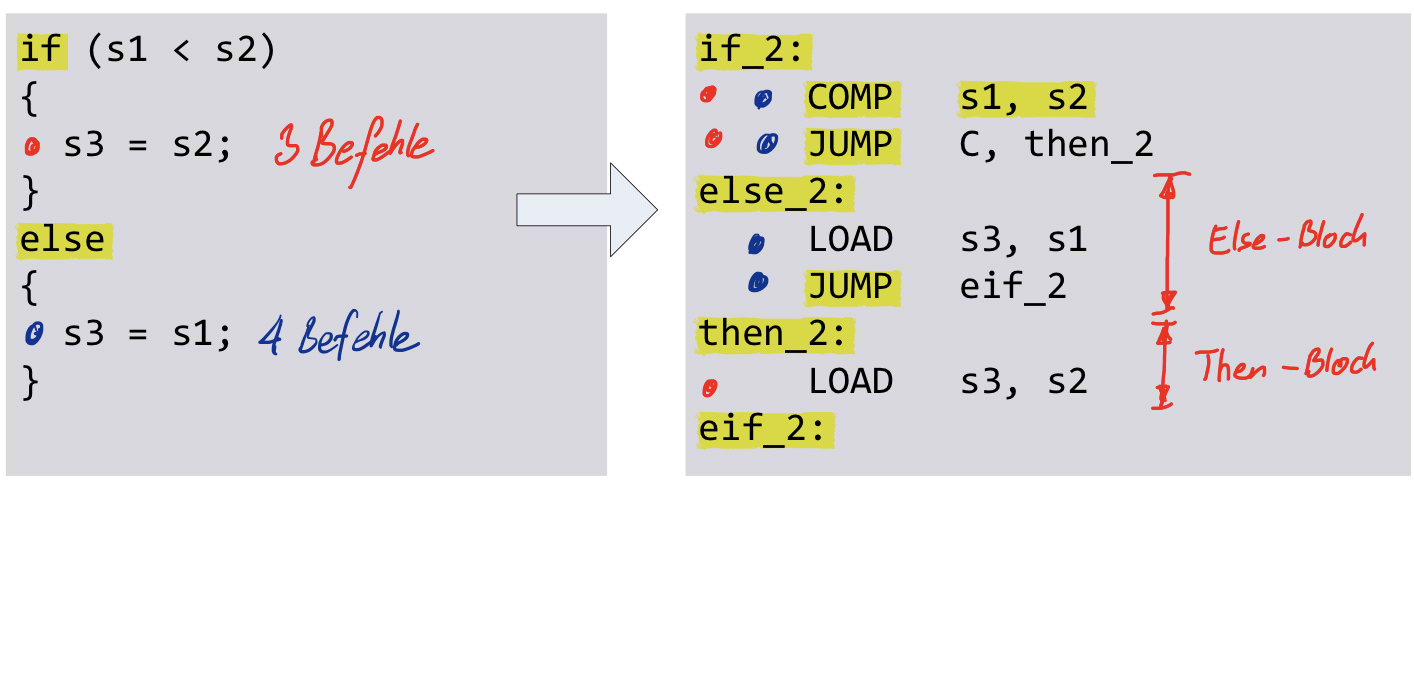
\includegraphics[width=8cm]{pics/Strukturierte_Programmierung}
\end{minipage}

\subsection{Unterprogrammverarbeitung}
\begin{minipage}{10cm}
	\subsubsection{Subroutine mit Parameter"ubergabe}
	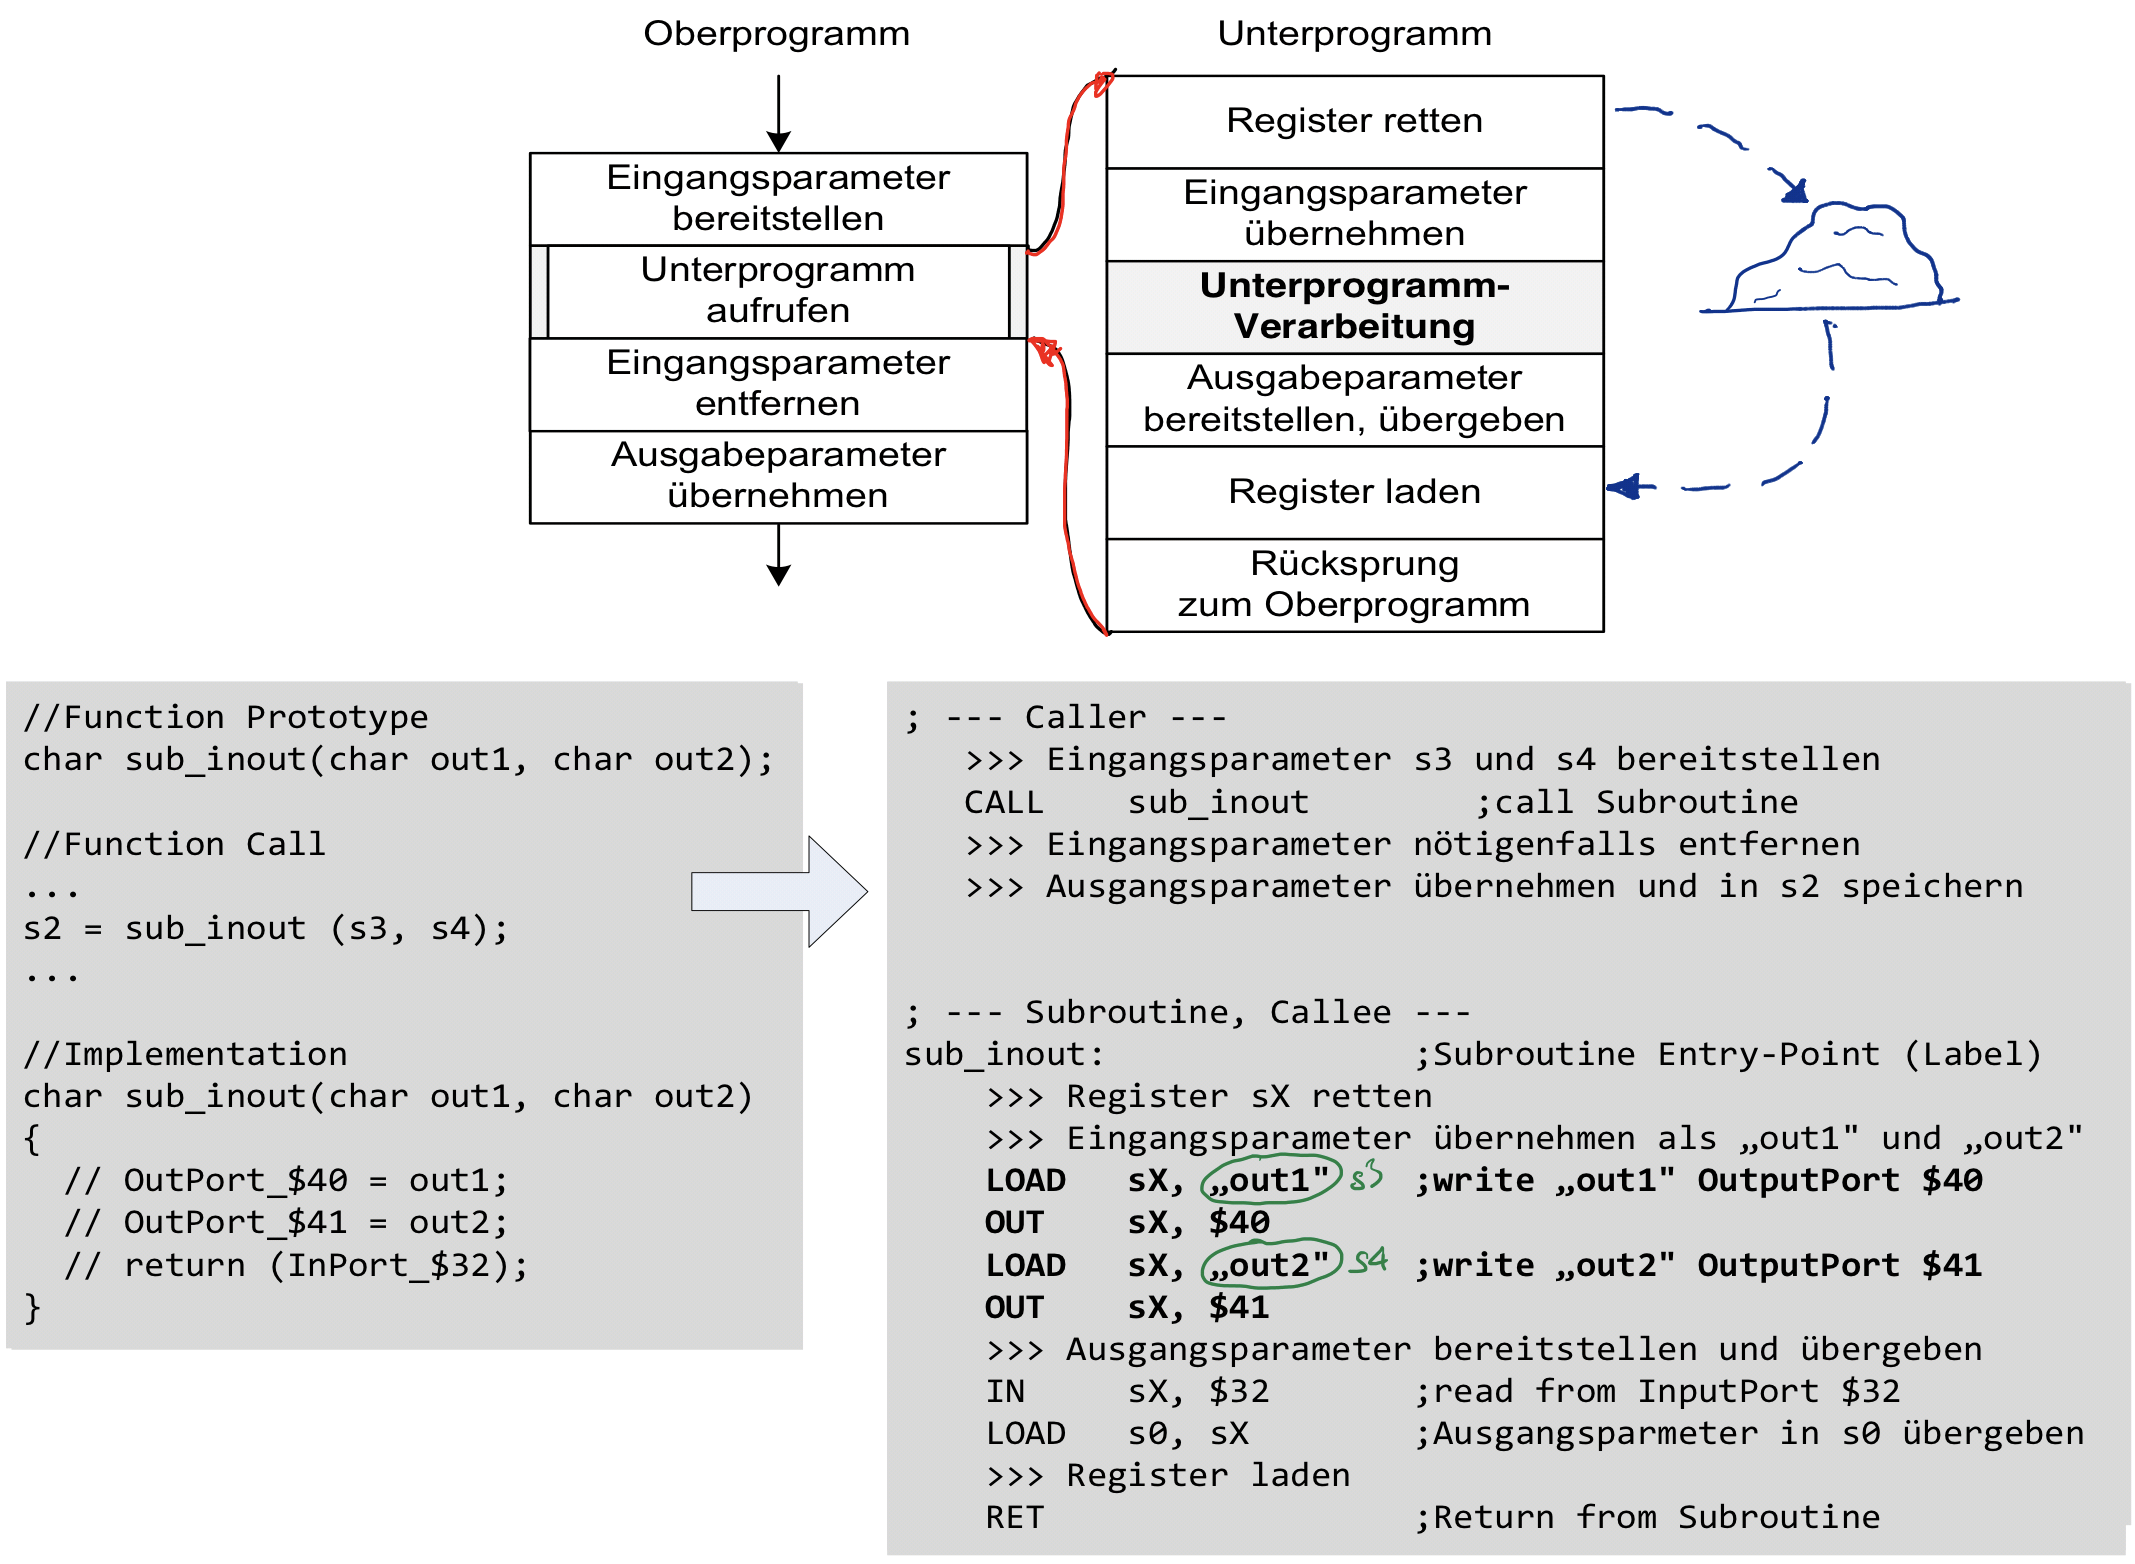
\includegraphics[width = 9.5cm]{pics/Subroutine_Mit_Parameter}
\end{minipage}
%
\begin{minipage}{0.5cm}
	\ \
\end{minipage}
%
\begin{minipage}{8cm}
	\subsubsection{Subroutine ohne Parameter"ubergabe}
	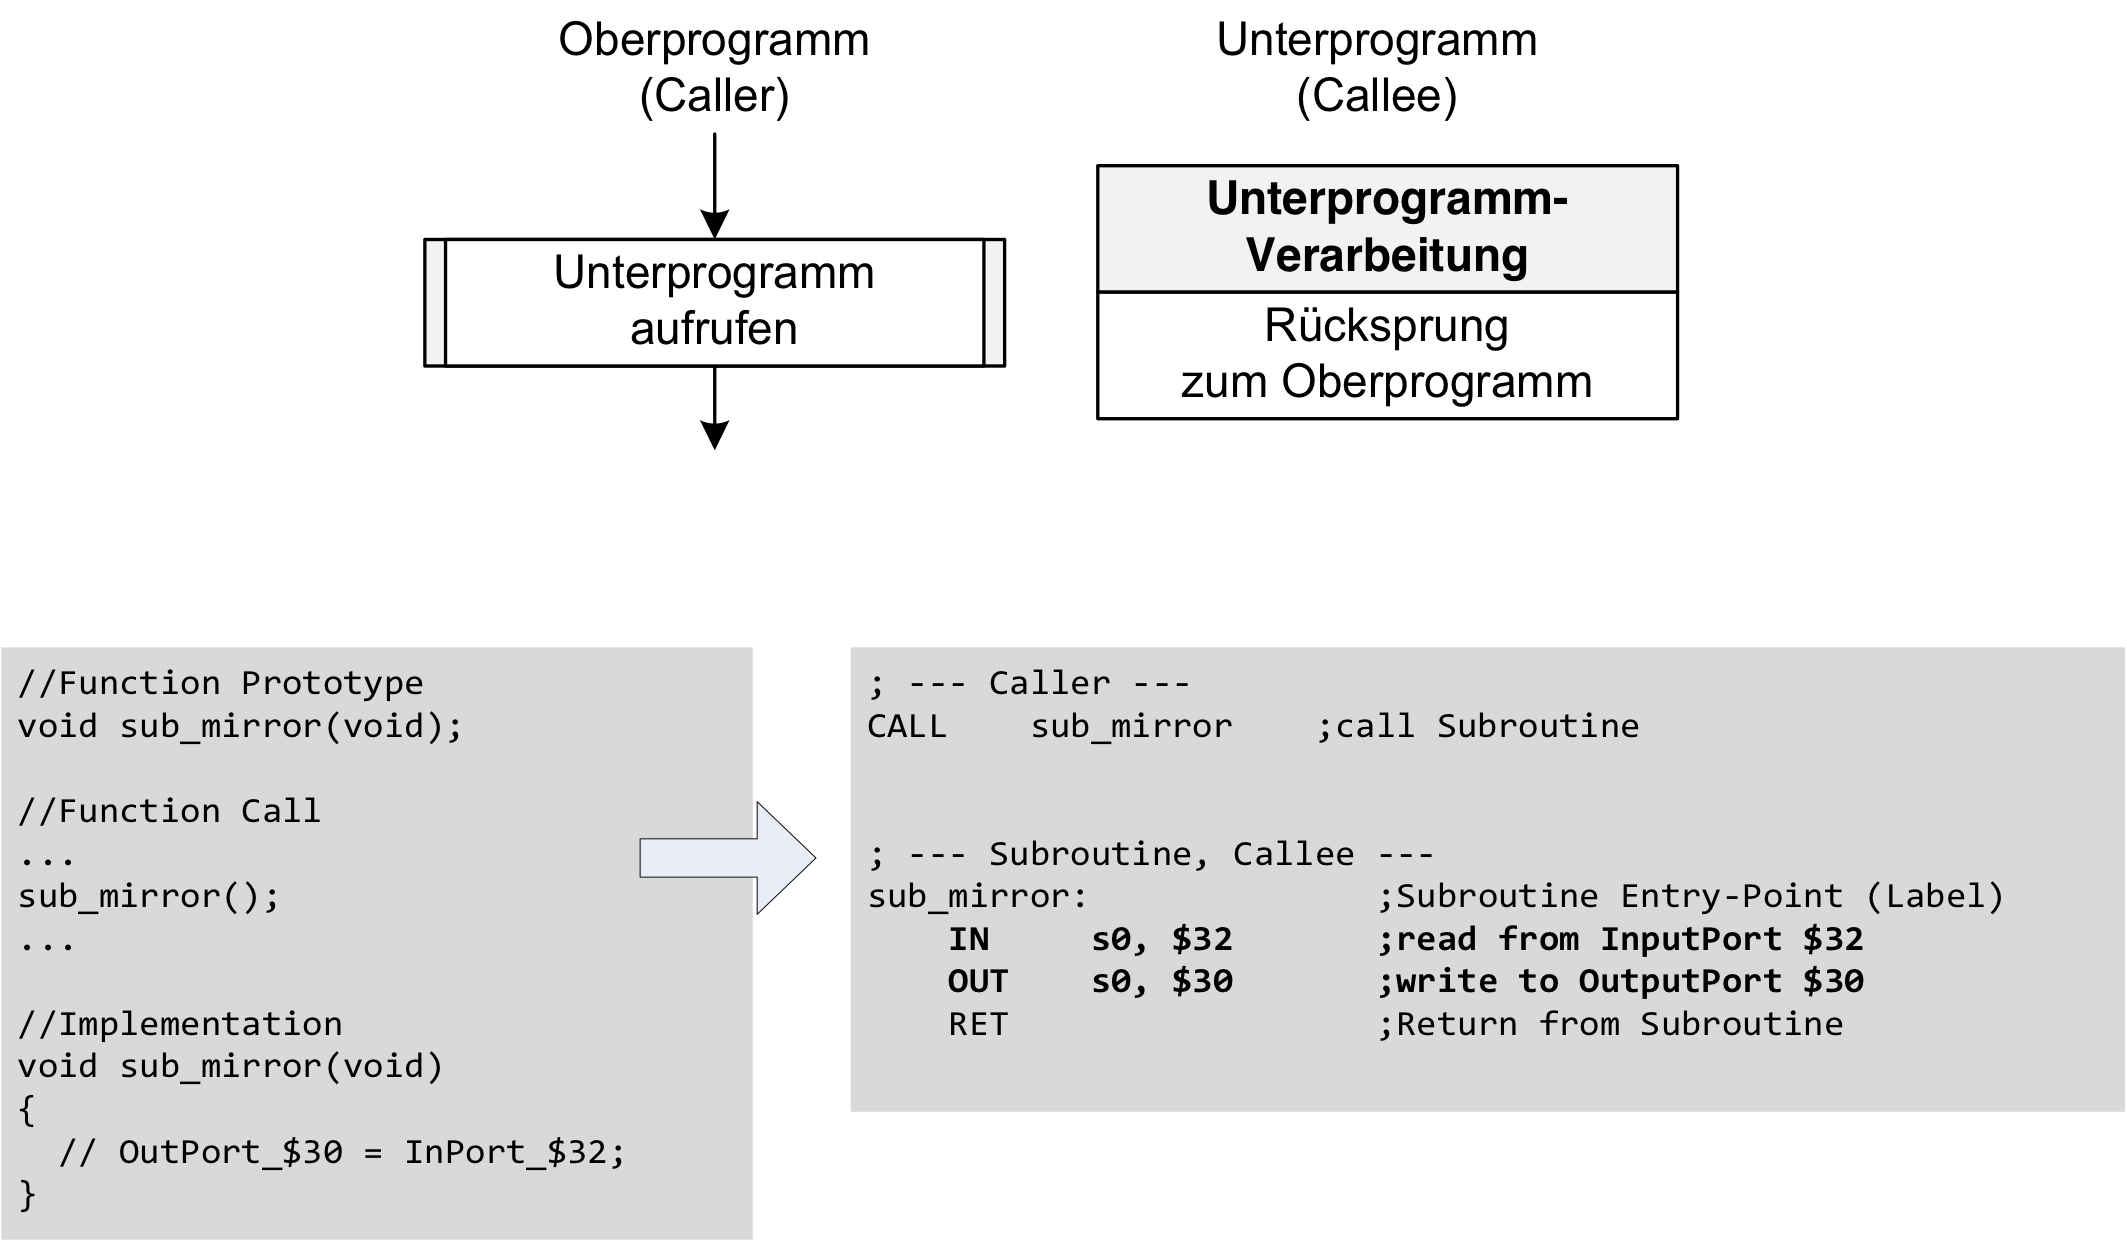
\includegraphics[width = 8cm]{pics/Subroutine_ohne_Parameter}
	
	Zu beachten ist das der PicoBlaze einen Call/Return-Stack besitzt welcher 31 Speicherstellen hat, das heisst es k"onnen 31 R"ucksprungsadressen gespeichert werden oder 31 Funktionen ineinander aufgerufen werden.
\end{minipage}

\subsection{Interrupts}
\begin{minipage}{10cm}
	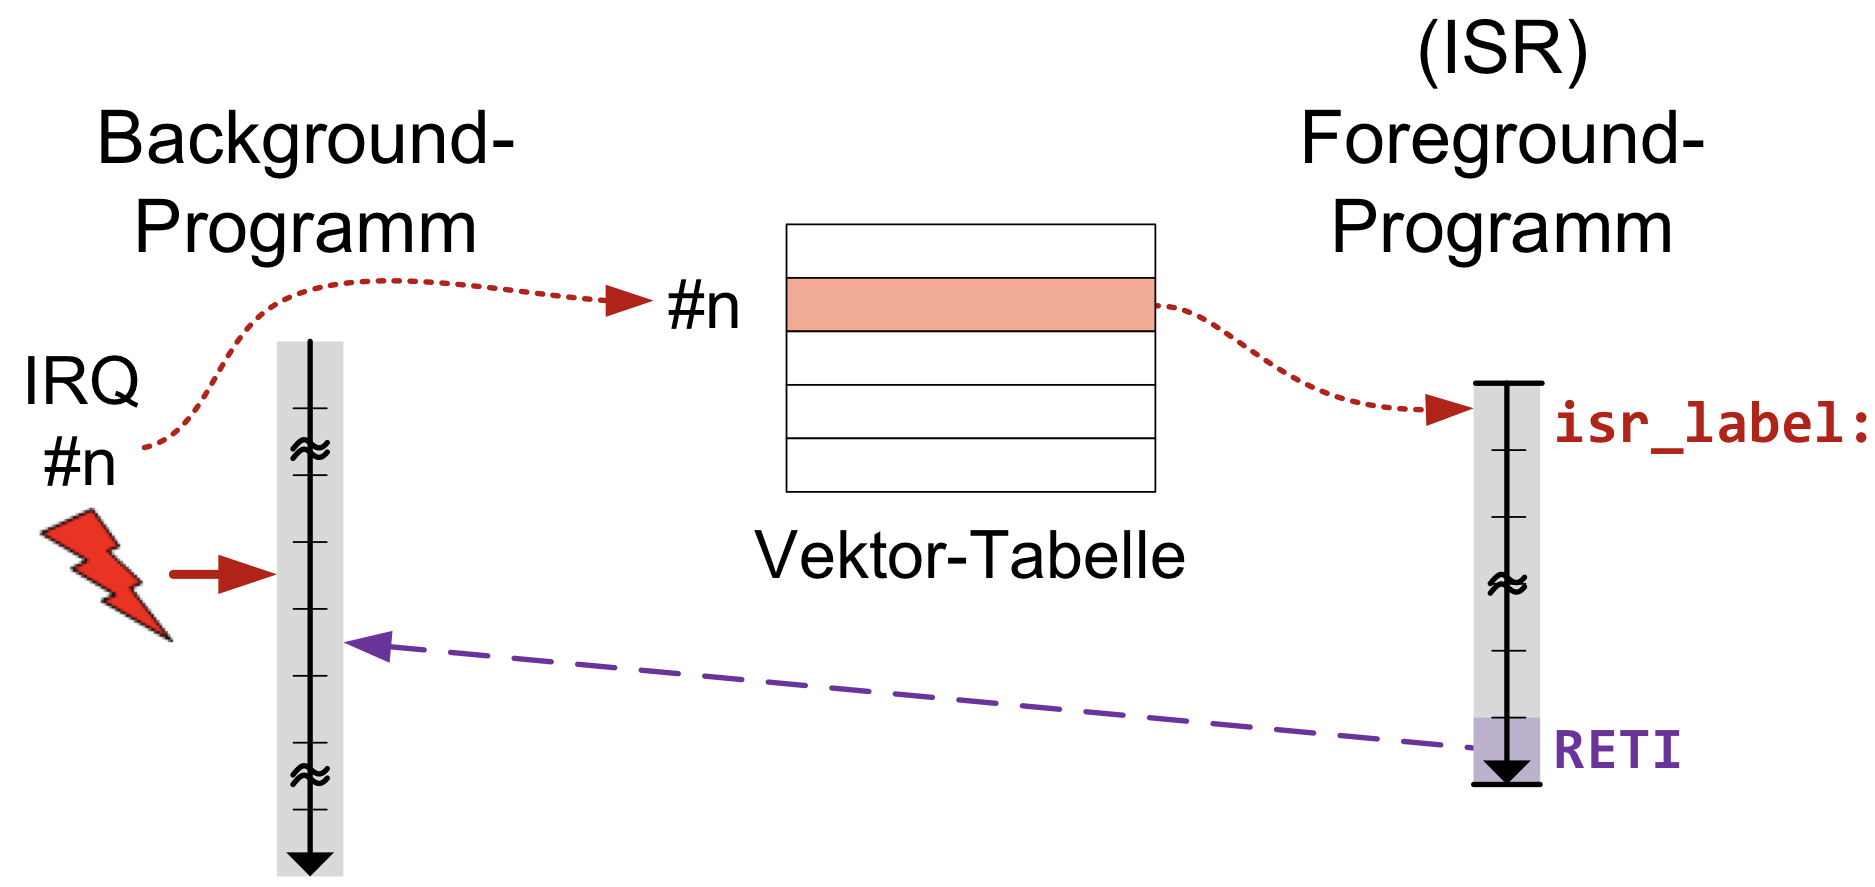
\includegraphics[width=6cm]{pics/Interrupt_Call}
	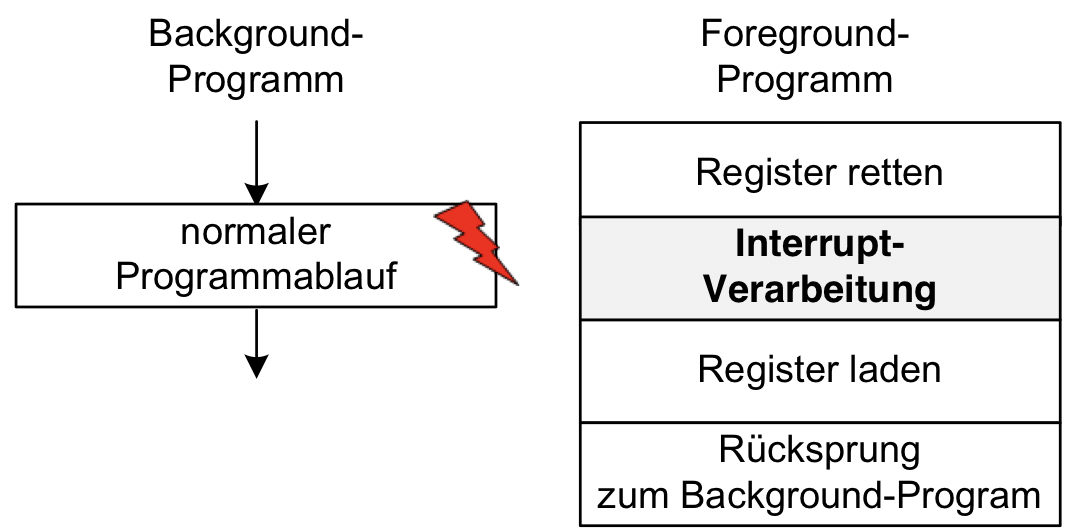
\includegraphics[width=5.5cm]{pics/Interrupt-Ablauf}
\end{minipage}
%
\begin{minipage}{0.5cm}
	\ \
\end{minipage}
%
\begin{minipage}{8cm}
	Der Interruptrequest (IRQ) erfolgt asynchron zum Programmablauf, wenn dieser auftritt wird mindestens noch der anstehende Befehl ausgef"uhrt. Durch die Interrupt-Vektor-Tabelle wird dan bestimmt welche Interruptserviceroutine (ISR) ausgef"uhrt wird, in der Tabelle stehen haupts"achlich JUMP-Befehle. Der PicoBlaze hat nur einen einzigen Interrupt-Vektor welcher sich an der Adresse \$3FF des Programmspeichers befindet. Es k"onnen keine Parameter an eine ISR "ubergeben werden, zudem m"ussen Interrupts mit \textbf{EINT} eingeschalten werden und am Ende der ISR wird entweder mit \textbf{RETI ENABLE/DISABLE} in den normalen Programmablauf zur"uckgekehrt.
\end{minipage}

\subsection{Transparenz-Grundsatz}
\begin{minipage}{10cm}
	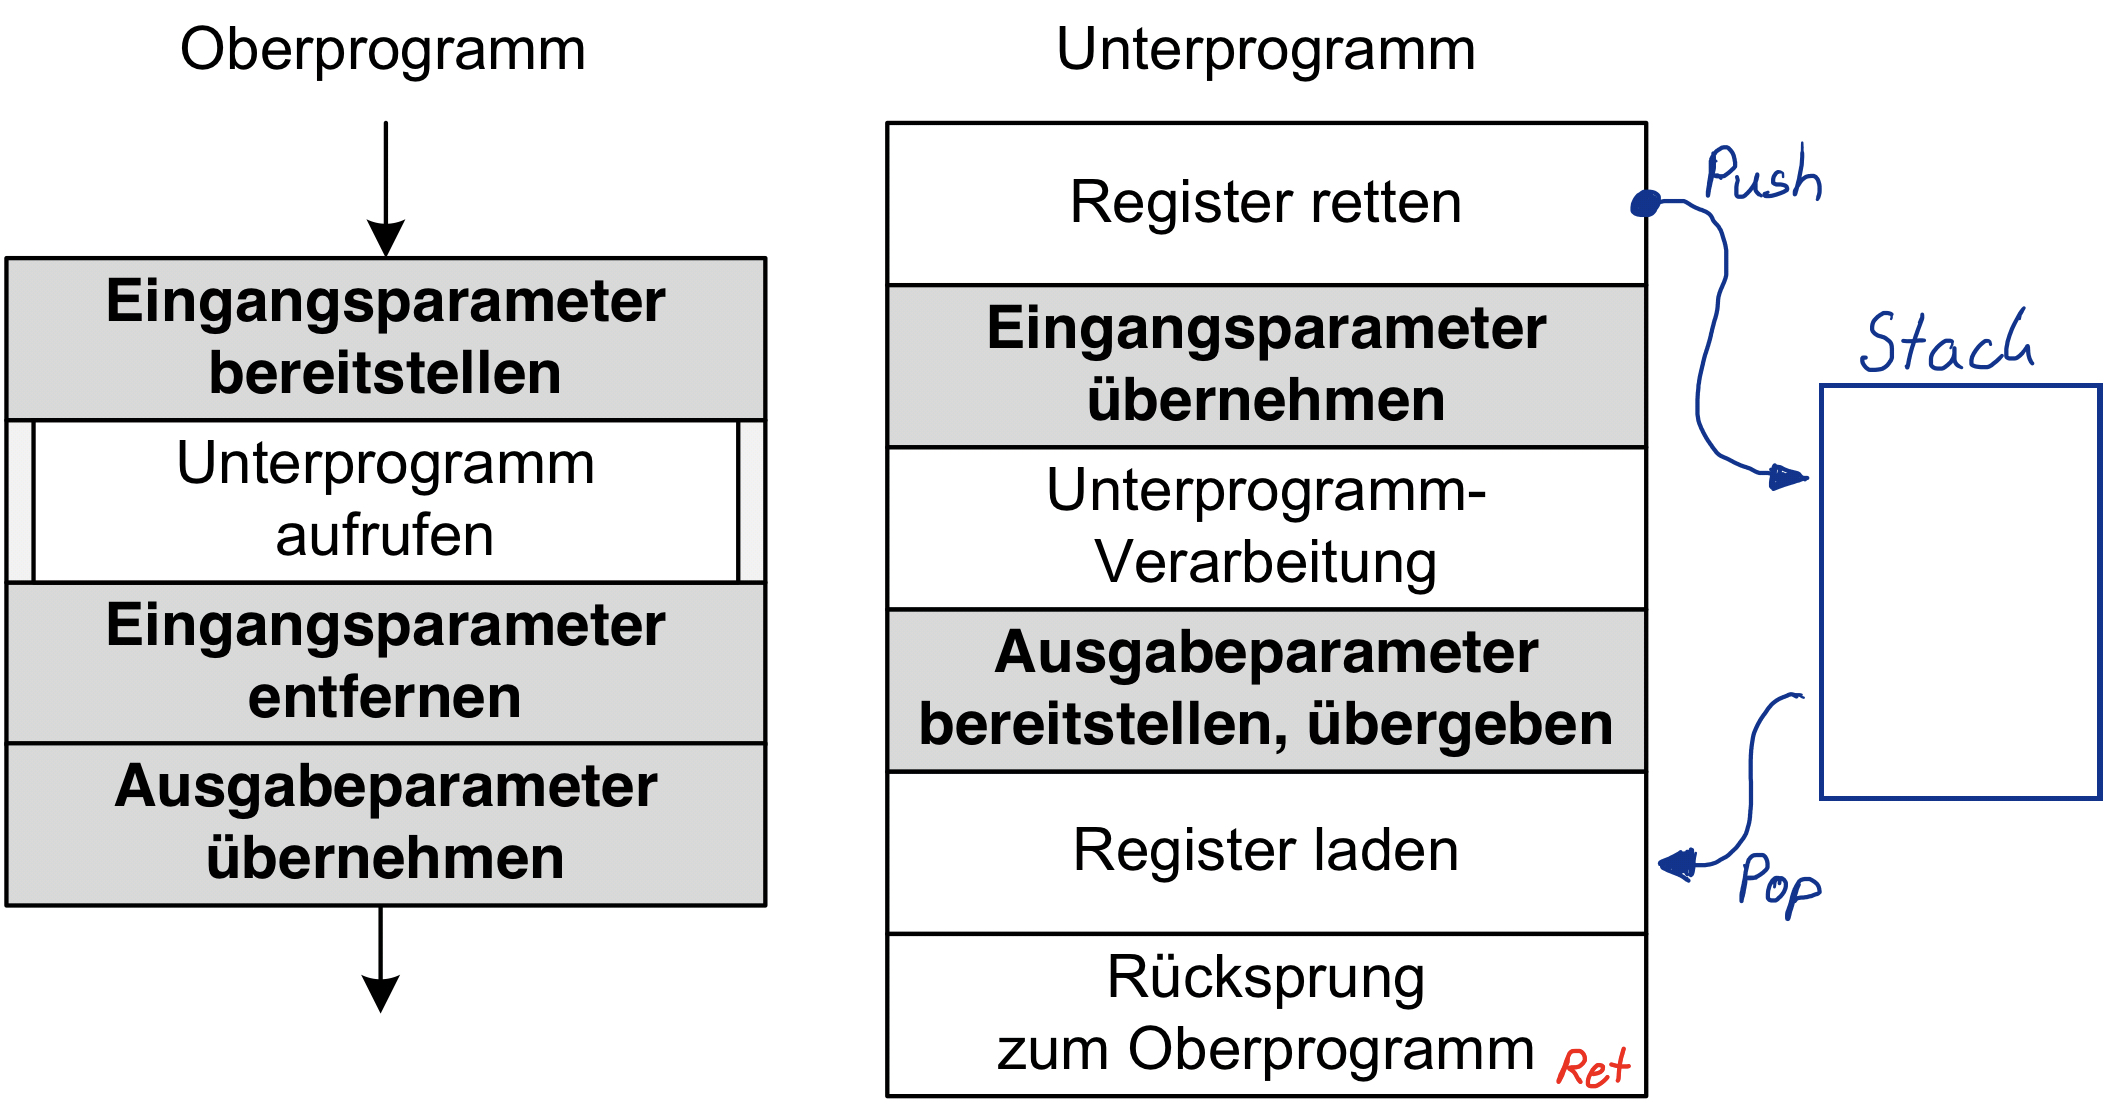
\includegraphics[width=6cm]{pics/Transparenz-Grundsatz}
\end{minipage}
%
\begin{minipage}{0.5cm}
	\ \
\end{minipage}
%
\begin{minipage}{8cm}
	Im Bezug auf Unterprogramm- und Interrupt-Verarbeitung sind sowohl Caller und Callee, bzw. Background- und Foreground-Programm beiderseits daf"ur verantwortlich, die verwendeten Ressourcen und Zust"ande stets so zu hinterlassen, wie diese vor der Verarbeitung angetroffen wurden
\end{minipage}

\subsection{Parameter"ubergabe nach C-Standard}
\begin{minipage}{9cm}
	Die Parameter"ubergabe mittels Stack entspricht dem C-Standard und verwendet ein klar definiertes, striktes Regime:
\begin{itemize}
	\item Die Parameter werden in der Reihenfolge von rechts-nach-links nacheinander auf den Stack gelegt. Die Parameter werden \textit{by value} oder \textit{by reference} "ubergeben.
	\item Der Return-Value (Funktionswert) wird in einem klar definierten Register an den Caller "ubergeben.
\end{itemize}
Da der PicoBlaze keinen Software-Stack hat, muss dieser noch vom Programmierer implementiert werden. Mit diesem und dem Transparenz-Grundsatz kann erreicht werden, dass der Code \textbf{reentrant} ist, das heisst das ein Interrupt w"ahrend einem Unterprogrammablauf dessen Werte nicht durcheinander bringt.
\end{minipage}
%
\begin{minipage}{0.5cm}
	\ \
\end{minipage}
%
\begin{minipage}{9cm}
	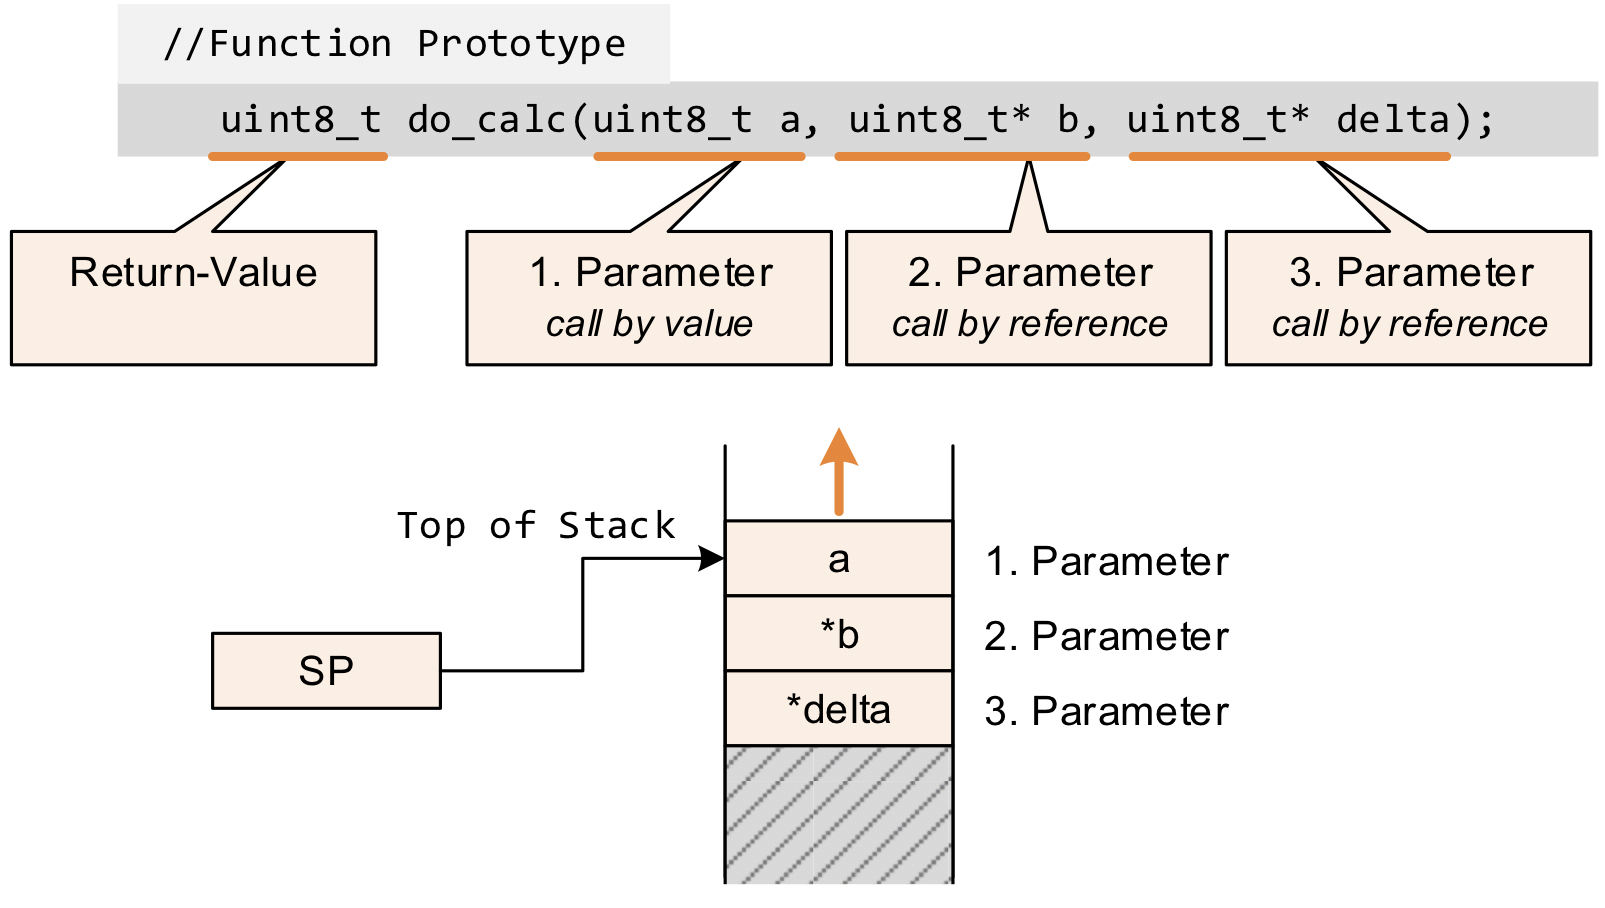
\includegraphics[width=9cm]{pics/Function_C-Standard}
\end{minipage}
